% ============================================================================
\section{Modern ASR}
% ============================================================================

\begin{frame}[plain]
  \centering
  \vspace{0.10\textheight}
  {\LARGE \textbf{Modern ASR}}

  \vspace{0.08\textheight}
  {\large Conformer encoders and Whisper-scale weak supervision\\define current practice}
\end{frame}

\begin{frame}{Conformer: Convolution-augmented Transformer}
  \begin{itemize}\footnotesize
    \item Sequence-to-sequence transformer with multi-headed self attention.
    \item Combines attention (global context) with convolution (local invariance).
    \item Uses RNN-T loss architecture.
  \end{itemize}
  \centering
  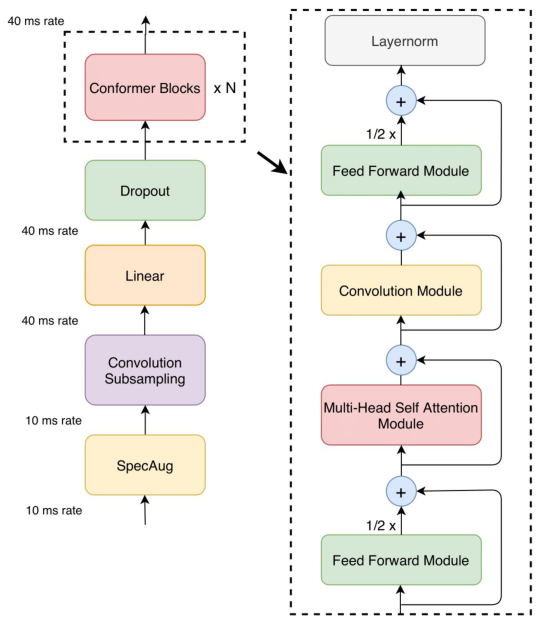
\includegraphics[width=\textwidth,height=0.46\textheight,keepaspectratio]{images/stt/stt_conformer_block_architecture.png}

  {\scriptsize Conformer encoder block: two macaron-like feed-forward layers with half-step residual connections sandwich the multi-headed self-attention and convolution modules, followed by a post layernorm.}
  \slideimgsource{Gulati et al., ``Conformer,'' Fig.~1; \href{https://arxiv.org/abs/2005.08100}{arXiv:2005.08100}.}
\end{frame}

\begin{frame}{SpecAugment: Augmenting data to increase dataset size}
  \begin{itemize}\footnotesize
    \item Three operations on the log-mel input during training: \textbf{time warping}, \textbf{frequency masking}, and \textbf{time masking}.
    \item Applied on the fly at the front of the encoder, so every epoch sees a different view of the same utterance.
  \end{itemize}
  \centering
  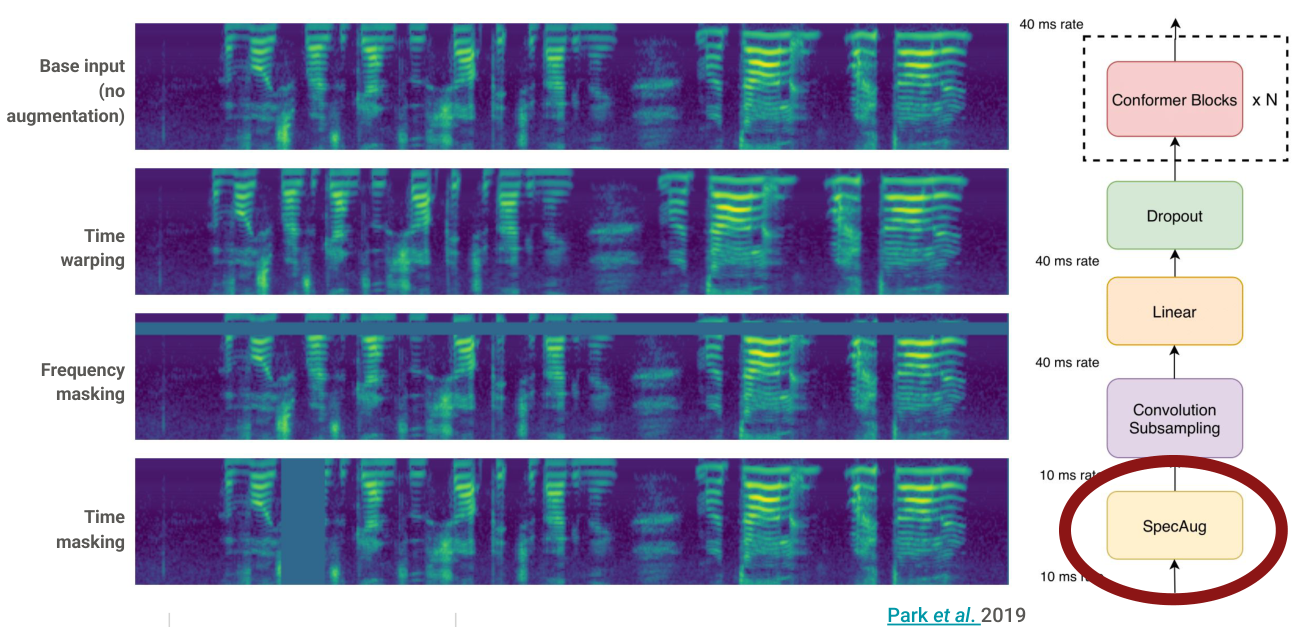
\includegraphics[width=\textwidth,height=0.62\textheight,keepaspectratio]{images/stt/stt_specaugment_spectrograms.png}
  \slideimgsource{Spectrograms: Park et al., ``SpecAugment,'' Fig.~1; \href{https://arxiv.org/abs/1904.08779}{arXiv:1904.08779}. Encoder pipeline: Gulati et al., Conformer, Fig.~1. Via Stanford CS224S, Lecture 11 (2025 Spring), slide 5.}
\end{frame}

\begin{frame}{Convolution subsampling: Log mel spectrogram is an image}
  \centering
  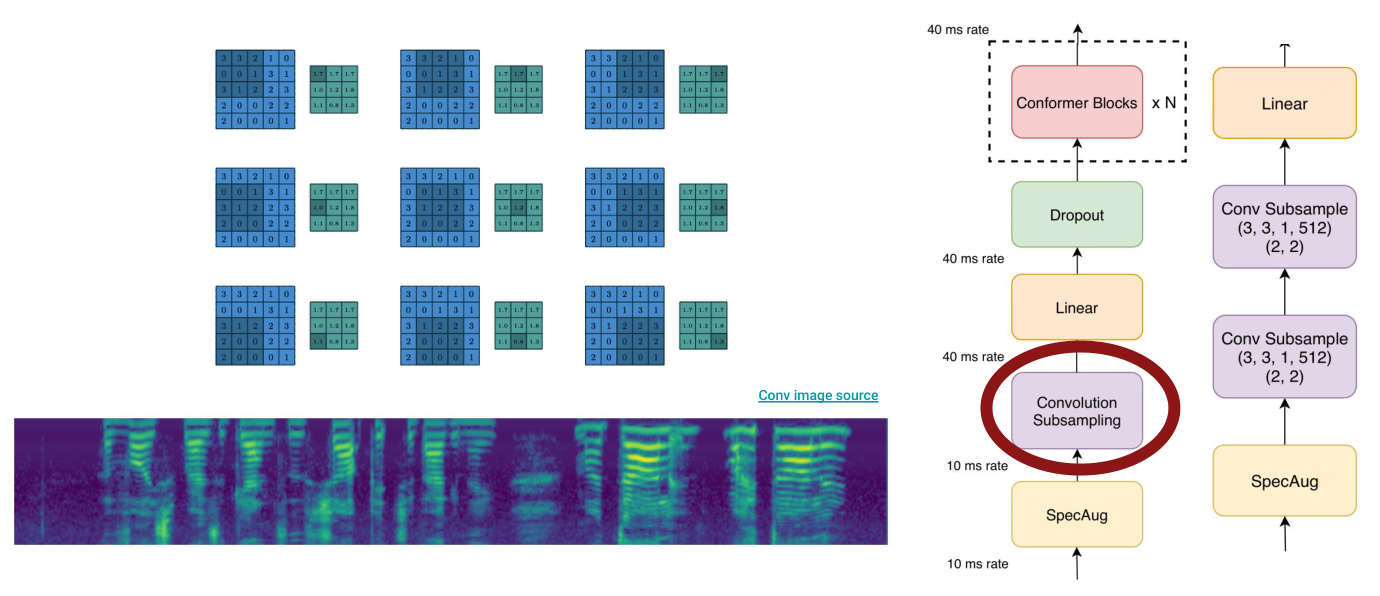
\includegraphics[width=\textwidth,height=0.70\textheight,keepaspectratio]{images/stt/stt_conformer_conv_subsampling.png}
  \slideimgsource{Grid animation: Dumoulin \& Visin, ``A guide to convolution arithmetic for deep learning,'' Fig.~1.5, which is a $3\times3$ \emph{average pooling} over a $5\times5$ input rather than a convolution; \href{https://arxiv.org/abs/1603.07285}{arXiv:1603.07285}. Encoder column: Gulati et al., Conformer, Fig.~1 (left panel); the conv-subsample expansion at right is CS224S's own. Via Stanford CS224S, Lecture 11 (2025 Spring), slide 6.}
\end{frame}


\begin{frame}{The convolution block matters most}
  \begin{columns}[c]
    \begin{column}{0.51\textwidth}
      \begin{itemize}\footnotesize
        \item From ablation experiment of the paper, \textbf{removing unique features and moving towards a vanilla Transformer block} was tested.
        \item Each row removes one more Conformer-specific component, cumulatively.
        \item All ablation study results are evaluated without external LM.
      \end{itemize}
    \end{column}
    \begin{column}{0.47\textwidth}
      \centering
      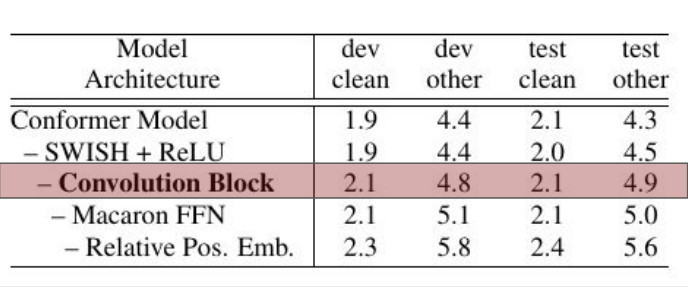
\includegraphics[width=\textwidth,height=0.72\textheight,keepaspectratio]{images/stt/stt_conformer_ablation_table.png}
      \slideimgsource{Gulati et al., ``Conformer,'' Table~3; \href{https://arxiv.org/abs/2005.08100}{arXiv:2005.08100}.}
    \end{column}
  \end{columns}
\end{frame}

\begin{frame}{State-of-the-art ASR: Whisper}
  \centering
  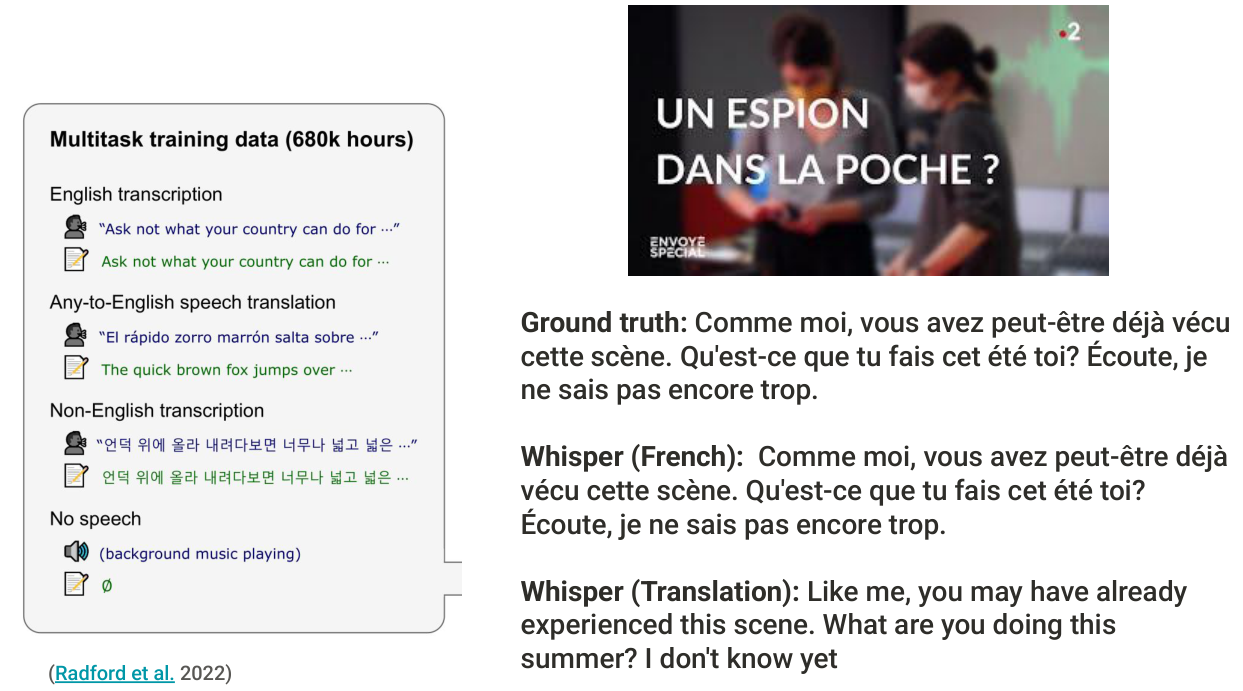
\includegraphics[width=\textwidth,height=0.82\textheight,keepaspectratio]{images/stt/stt_whisper_multilingual_example.png}
  \slideimgsource{Training-data panel: Radford et al., Whisper, Fig.~1; \href{https://arxiv.org/abs/2212.04356}{arXiv:2212.04356}. Video still: France~2, \textit{Envoy\'e Sp\'ecial}. Via Stanford CS224S, Lecture 11 (2025 Spring), slide 18.}
\end{frame}

\begin{frame}{Whisper: How does it perform a variety of tasks accurately?}
  \centering
  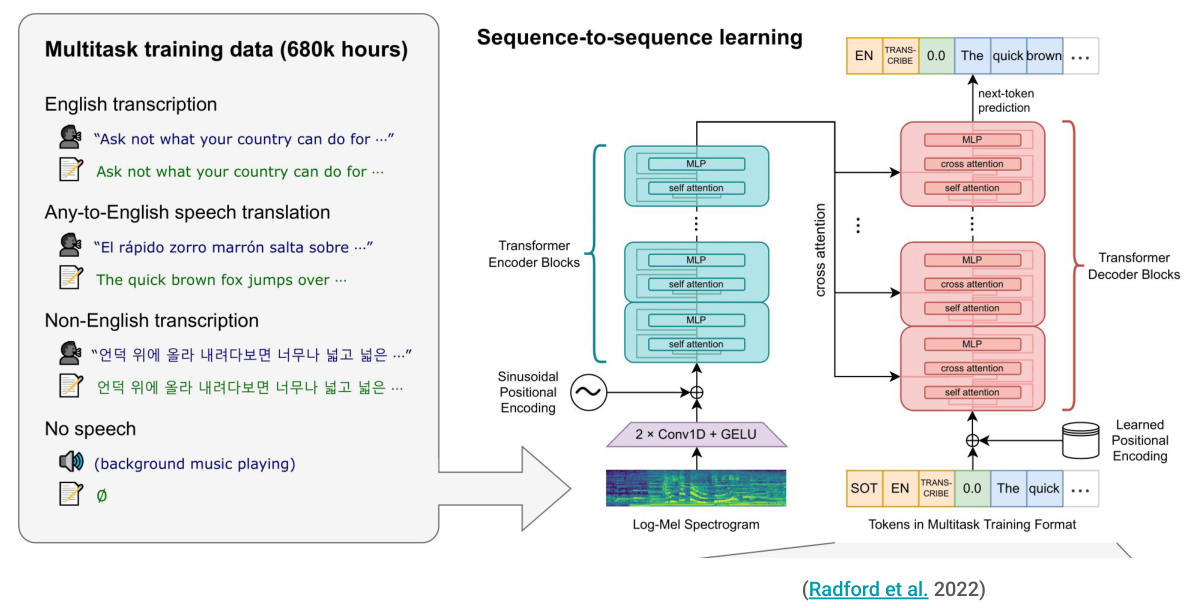
\includegraphics[width=\textwidth,height=0.84\textheight,keepaspectratio]{images/stt/stt_whisper_multitask_seq2seq.png}
  \slideimgsource{Radford et al., Whisper, Fig.~1 (``Overview of our approach''); \href{https://arxiv.org/abs/2212.04356}{arXiv:2212.04356}.}
\end{frame}

\begin{frame}{Whisper: encoder--decoder architecture}
  \centering
  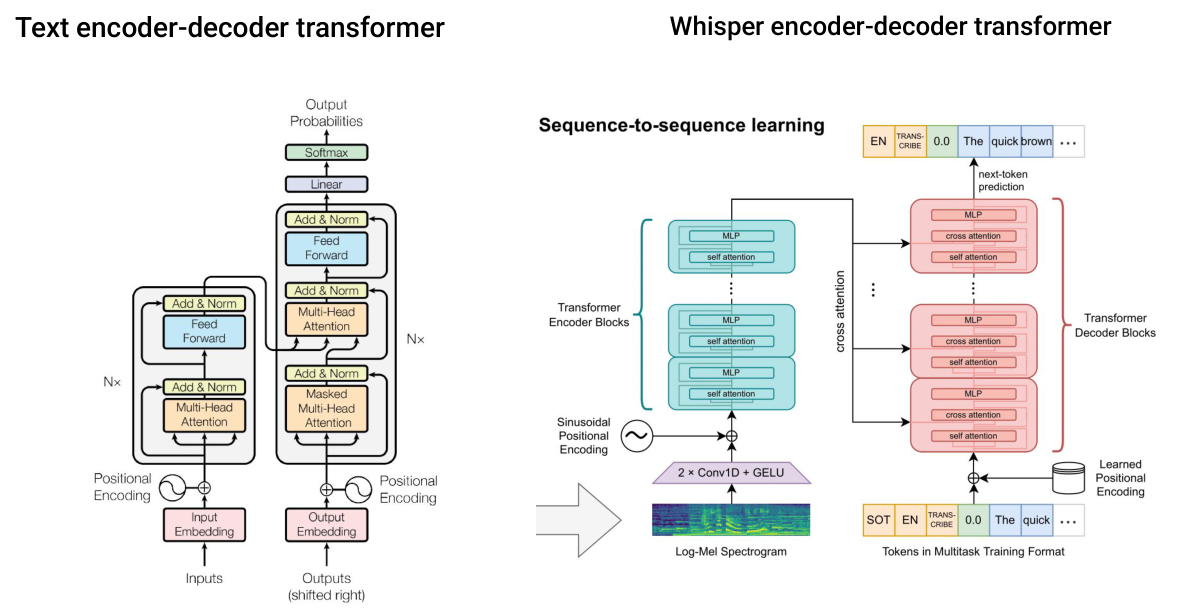
\includegraphics[width=\textwidth,height=0.82\textheight,keepaspectratio]{images/stt/stt_whisper_vs_text_transformer.png}
  \slideimgsource{Left: Vaswani et al., ``Attention Is All You Need,'' Fig.~1; \href{https://arxiv.org/abs/1706.03762}{arXiv:1706.03762}. Right: Radford et al., Whisper, Fig.~1; \href{https://arxiv.org/abs/2212.04356}{arXiv:2212.04356}.}
\end{frame}

\begin{frame}{Whisper encoder}
  \begin{columns}[c]
    \begin{column}{0.41\textwidth}
      \raggedright
      \textbf{\textcolor{KAred}{Whisper encoder:}\\ transformer encoder}
      \begin{itemize}
        \item Encoder input: log-mel spectrogram and two convolutional layers
        \item Sinusoidal positional encoding
        \item Standard transformer blocks depending on model size
      \end{itemize}
    \end{column}
    \begin{column}{0.58\textwidth}
      \centering
      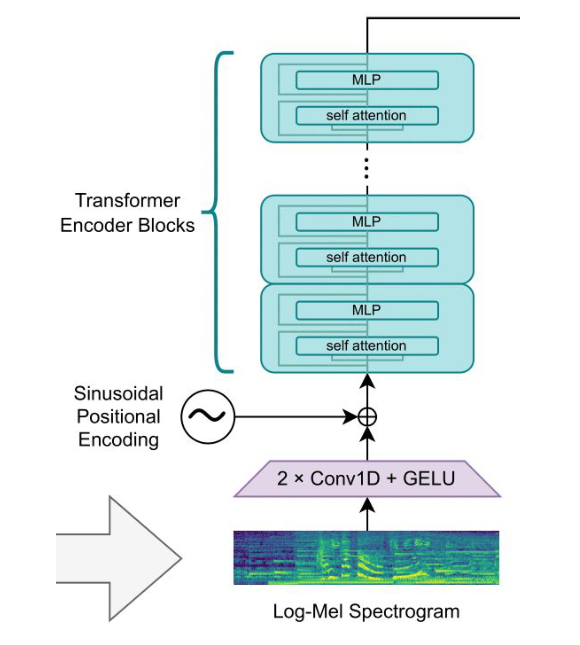
\includegraphics[width=0.5\textwidth,height=0.60\textheight,keepaspectratio]{images/stt/stt_whisper_encoder_detail.png}
      \slideimgsource{Radford et al., Whisper, Fig.~1 (encoder panel); \href{https://arxiv.org/abs/2212.04356}{arXiv:2212.04356}.}
    \end{column}
  \end{columns}
\end{frame}

\begin{frame}{Whisper decoder: autoregressive transformer decoder}
  \begin{columns}[c]
    \begin{column}{0.48\textwidth}
      \raggedright
      \begin{itemize}
        \item \textbf{GPT-2 style} model: no more CTC loss.
        \item Decodes using \textbf{auto-regressive prediction}: each token depends on previous (\texttt{text} prediction).
        \item \textbf{Cross-attention:} To encoded audio representation from encoder.
        \item \textbf{Custom vocabulary and tags:}
        \begin{itemize}
            \item Language tags: \texttt{<en>}, \texttt{<fr>}, etc.
            \item Task tags: \texttt{<transcribe>}, \texttt{<translate>}
            \item \textbf{Timestamps}
            \item Speech tags: \texttt{<nospeech>}
        \end{itemize}
      \end{itemize}
    \end{column}
    \begin{column}{0.51\textwidth}
      \centering
      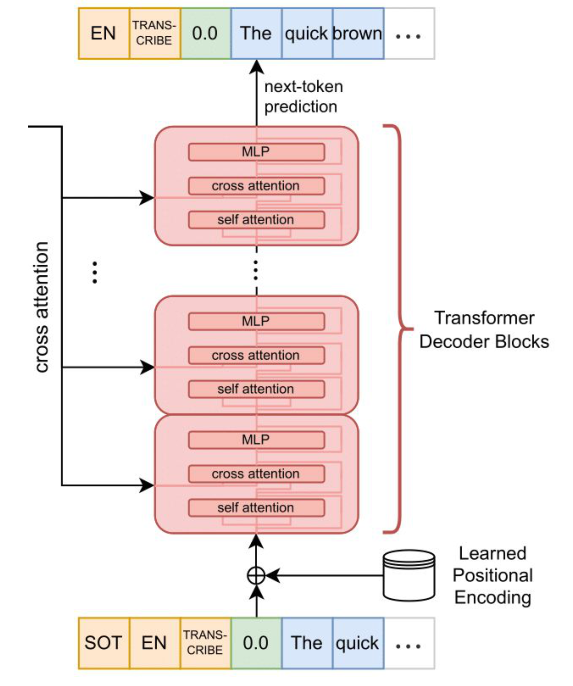
\includegraphics[width=\textwidth,height=0.80\textheight,keepaspectratio]{images/stt/stt_whisper_decoder_detail.png}
      \slideimgsource{Radford et al., Whisper, Fig.~1 (decoder panel); \href{https://arxiv.org/abs/2212.04356}{arXiv:2212.04356}.}
    \end{column}
  \end{columns}
\end{frame}

\begin{frame}{Whisper handles long-form transcription}
  \begin{columns}[T]
    \begin{column}{0.40\textwidth}
      \begin{itemize}\footnotesize
        \item Whisper only takes 30 seconds of speech at a time
        \item \textbf{Timestamp tokens} are used to determine when to shift the window
        \item Text from the previous window is provided with transcribing current window
        \item Voice activity detection using the \texttt{\textless{}nospeech\textgreater{}} tag
      \end{itemize}
    \end{column}
    \begin{column}{0.60\textwidth}
      \centering
      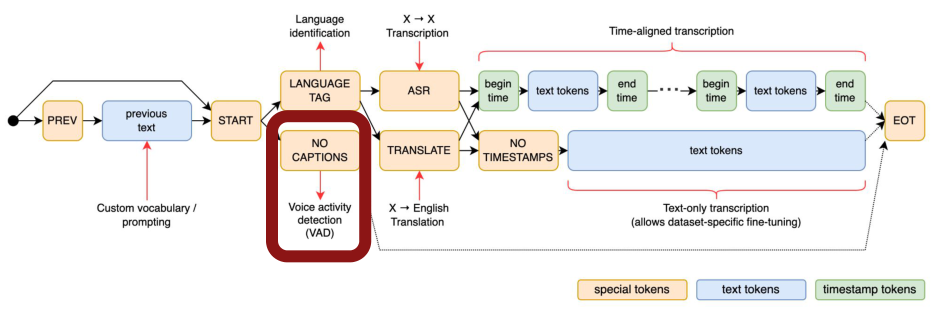
\includegraphics[width=\textwidth,keepaspectratio]{images/stt/stt_whisper_token_sequence_format.png}
      \slideimgsource{Stanford CS224S, Lecture 11 (2025 Spring), slide 30: a redraw of Radford et al., Whisper, Fig.~1 (multitask training format), with the VAD branch ringed in red by the lecturer. The published figure reads \texttt{START OF TRANSCRIPT}, \texttt{NO SPEECH} and \texttt{TRANSCRIBE}; \href{https://arxiv.org/abs/2212.04356}{arXiv:2212.04356}.}
    \end{column}
  \end{columns}
\end{frame}

\begin{frame}{Whisper's automatic speech translation performance}
  \begin{columns}[T]
    \begin{column}{0.48\textwidth}
    \centering
    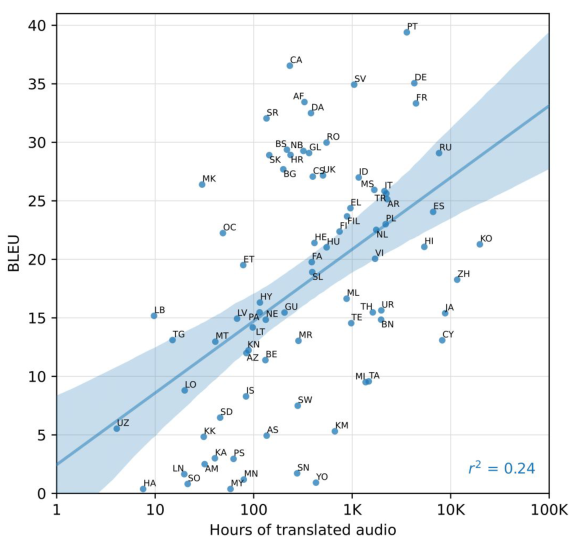
\includegraphics[width=\textwidth,keepaspectratio]{images/stt/stt_whisper_translation_bleu_scaling.png}
    \slideimgsource{Radford et al., Whisper, Fig.~4; \href{https://arxiv.org/abs/2212.04356}{arXiv:2212.04356}.}
    \end{column}
    \begin{column}{0.50\textwidth}
      \textbf{Speech translation performance on FLEURS dataset (higher is better)}
      \begin{itemize}
        \item Translation performance is better on average after the 100 hours of training data mark.
        \item Amount of training data isn't as correlated with translation performance as it is with transcription performance.
        \item Although possible, speech translation is likely to only be reliable for high resource languages.
      \end{itemize}
    \end{column}
  \end{columns}
\end{frame}

\begin{frame}{Where Whisper still fails}
  \begin{itemize}\footnotesize
    \item Scale steadily reduced \textbf{perception-level} errors such as confusing similar-sounding words. What remains the paper calls ``decidedly non-human/perceptual'', and it bites hardest in long-form transcription.
    \item Three named failure modes, arising from the interaction of seq2seq decoding, the language model, and text-audio alignment:
      \begin{itemize}
        \item getting stuck in \textbf{repeat loops}
        \item failing to transcribe the \textbf{first or last few words} of a segment
        \item \textbf{complete hallucination}, where the output is a transcript entirely unrelated to the audio
      \end{itemize}
    \item These outputs are fluent, so they do not look like errors. Anything downstream that trusts the transcript inherits them silently.
    \item Coverage is uneven: the pre-training mix is English-heavy and most languages have under 1000 hours, so per-language accuracy tracks per-language data volume.
  \end{itemize}
  \slideimgsource{Radford et al., Whisper, \S6 ``Limitations and Future Work''; \href{https://arxiv.org/abs/2212.04356}{arXiv:2212.04356}.}
\end{frame}
